% NEUTRONICS BEAMER TEMPLATE -- START EDITING IN LINE 90
\documentclass[xcolor=x11names, compress, handout]{beamer}
%\documentclass[xcolor=x11names, compress]{beamer}
\usepackage{pgfpages}
\usepackage{algorithm}
\usepackage{algpseudocode}
\usepackage{appendixnumberbeamer}
\usepackage{booktabs}
\usepackage{amsmath}
\usepackage{tikz}
\usepackage{xcolor}
\usepackage[super]{nth}
\usepackage{sty/commands}
\usepackage{appendixnumberbeamer}
\usepackage{hyperref}
% \usepackage{array}


\definecolor{CoolBlack}{rgb}{0.0, 0.18, 0.39}
\definecolor{byellow}{rgb}{0.55037, 0.38821, 0.06142}

\usetikzlibrary{decorations.fractals}

\setbeamerfont{title like}{shape=\scshape}
\setbeamerfont{frametitle}{shape=\scshape}

\setbeamercolor*{lower separation line head}{bg=CoolBlack}
\setbeamercolor*{normal text}{fg=black,bg=white}
\setbeamercolor*{alerted text}{fg=dgreen} 
\setbeamercolor*{example text}{fg=black}
\setbeamercolor*{structure}{fg=black}

\setbeamertemplate{bibliography item}{\insertbiblabel}
% Margins
\mode<presentation>
{
  % \definecolor{berkeleyblue}{HTML}{003262}
  % \definecolor{berkeleygold}{HTML}{FDB515}
  \definecolor{berkeleyblue}{HTML}{FF7F00}
  \definecolor{berkeleygold}{HTML}{808080}
  \usetheme{Boadilla}      % or try Darmstadt, Madrid, Warsaw, Boadilla...
  % \usecolortheme{dove} % or try albatross, beaver, crane, ...
  \setbeamercolor{structure}{fg=berkeleyblue,bg=berkeleygold}
  \setbeamercolor{palette primary}{fg=berkeleyblue,bg=berkeleygold}
  \setbeamercolor{palette secondary}{fg=berkeleyblue,bg=berkeleygold}
  \setbeamercolor{palette tertiary}{bg=berkeleyblue,fg=white}
  \usefonttheme{structurebold}  % or try serif, structurebold, ...
  \useinnertheme{circles}
  \setbeamertemplate{caption}[numbered]
  \usebackgroundtemplate{}
}

%% Beamer Layout %%%%%%%%%%%%%%%%%%%%%%%%%%%%%
\useoutertheme[subsection=false,shadow]{miniframes}
%\useinnertheme{default}
%\usefonttheme{serif}
%\usepackage{palatino}
%\usepackage{tabu}
% addition of color
\definecolor{dgreen}{rgb}{0.,0.6,0.}
\definecolor{RawSienna}{cmyk}{0,0.72,1,0.45}
%\usepackage[sorting=none]{biblatex}
\mode<presentation>

% Links
\definecolor{links}{HTML}{003262}
\hypersetup{colorlinks,linkcolor=,urlcolor=links}

% columns
\renewcommand{\(}{\begin{columns}}
\renewcommand{\)}{\end{columns}}
\newcommand{\<}[1]{\begin{column}{#1}}
\renewcommand{\>}{\end{column}}


% Show table of content before each section
\AtBeginSection[]{
  \AtBeginSection[]{
  \begin{frame}[noframenumbering, plain]
  \frametitle{Outline}                     
  \centering
  \begin{minipage}[t][0.5\textheight]{0.75\textwidth}
    \linespread{2.0}
    \tableofcontents[currentsection]
  \end{minipage}
  \end{frame}
  }
}

% 
%THIS IS THE TITLE OF THE TALK
\title{Research Update}

%FEEL FREE TO EDIT THE COVER LAYOUT AS NEEDED
\author{Su-Ann Chong}

\date{June \nth{5}, 2020}


\begin{document}

\begin{frame}[plain]
  %THIS IS THE TITLE OF THE TALK
  \title{Research Updates:\\\large{High Rate Pixelated Neutron Detector}}

  %FEEL FREE TO EDIT THE COVER LAYOUT AS NEEDED
  \author{Su-Ann Chong}
  \institute{Monthly Group Meeting}
  % \institute{University of Tennessee, Knoxville/ Nuclear Engineering Department}
  \date{June \nth{5}, 2020}
  \titlepage
\end{frame}

%----------------------------------------------------------%
% WHEN YOU START A NEW SECTION, IT WILL SHOW UP AS A CLICKABLE
% SHORTCUT AT THE TOP OF YOUR FRAMES

\begin{frame}
  \frametitle{Outline}
  %\hfill                        
  \centering
  \begin{minipage}[t][0.5\textheight]{0.75\textwidth}
   \linespread{2.0}
   \tableofcontents
 \end{minipage}
  % \parbox{0.73\textwidth}{
  %   \tableofcontents
  %   }
\end{frame}


\section{\scshape Introduction}
\begin{frame}
  \frametitle{Neutron Reflectometry (NREF)}
  Neutron reflectometry is a neutron scattering technique that makes use of the reflection of neutrons to probe and analyze interfacial structure and composition. \\

  \begin{columns}
  \begin{column}{0.5\textwidth}
  Capability:
  \begin{itemize}
  \item{Specular reflectivity:} \\
        Depth profiles
  \item{Off-specular reflectivity:} \\
        Surface roughness
  \item{Glancing incidence diffraction:} \\
        Atomic structure near the surface
  \end{itemize}
  \end{column}
  \begin{column}{0.5\textwidth}  %%<--- here
  \begin{center}
  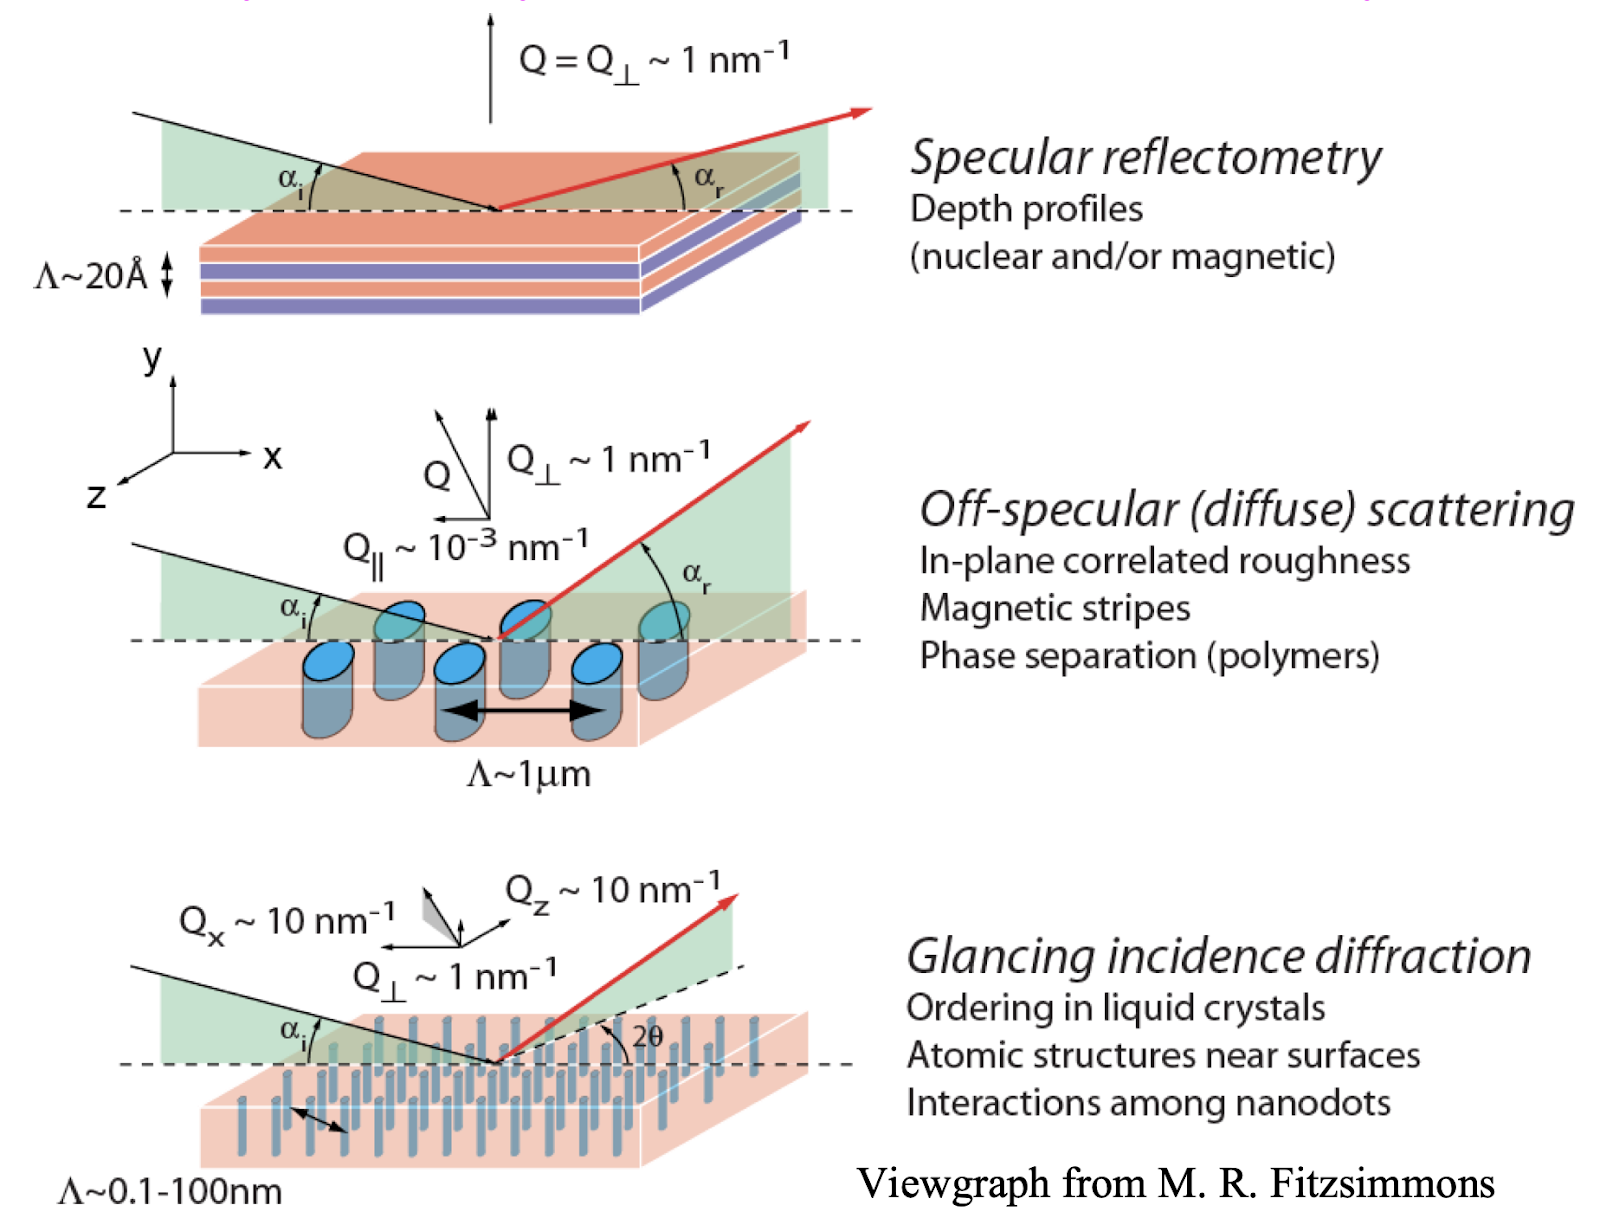
\includegraphics[width=\textwidth]{images/NREF_types.png}

  \end{center}
  \end{column}
  \end{columns}

\end{frame}

\begin{frame}
  \frametitle{Motivation}

  \begin{columns}
  \begin{column}{0.5\textwidth}
  Reasons:
  \begin{itemize}
  \item Increasing neutron flux in upcoming instruments
  \item Current detector technology lacks in counting rate capability
  \end{itemize}
  \begin{center}
  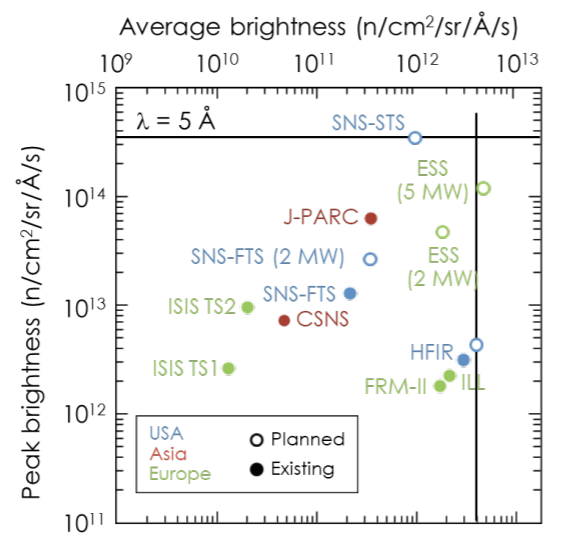
\includegraphics[width=0.7\textwidth]{images/neutron_sources.png}
  \end{center}
  \end{column}

  \begin{column}{0.5\textwidth}  %%<--- here
  \begin{center}
  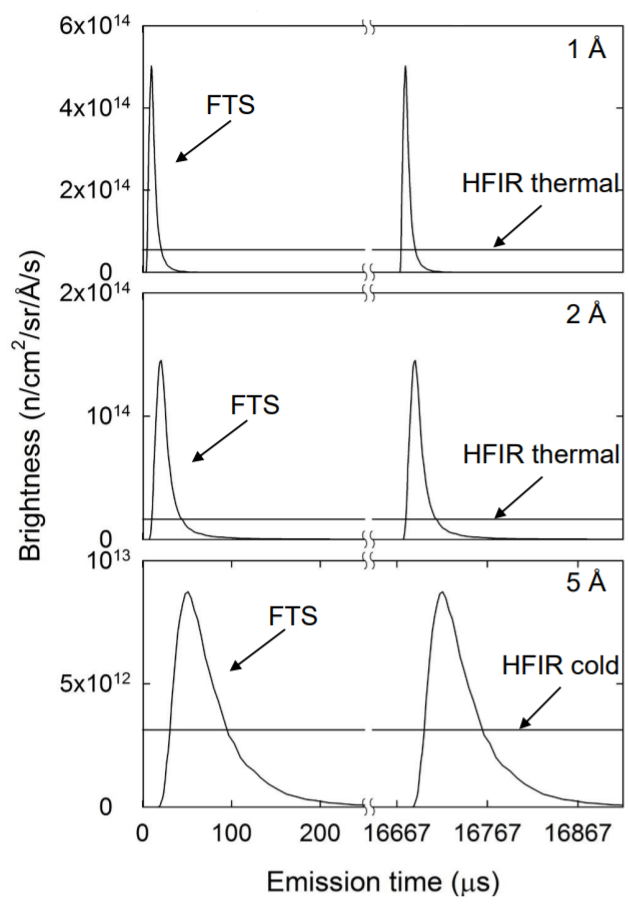
\includegraphics[width=0.9\textwidth]{images/reactor_SNS_pulses.png}
  \end{center}
  \end{column}
  \end{columns}

\end{frame}


\begin{frame}
  \frametitle{Project Goals}
  \begin{columns}
  \begin{column}{0.45\textwidth}
  The detector requirements for neutron reflectometers at ORNL are summarized here. \\
  \

  The project goal is to aim to satisfy all aspects of the requirements, except the active area of the detector.\\ 
  \

  \end{column}

  \begin{column}{0.5\textwidth}  %%<--- here
  \begin{block}{Detector Requirement}
  \begin{center}
  \begin{tabular}{l c}
  \hline
  Parameter & Desired \\
  \hline
  Counting rate & 1 MHz/cm$^2$\\
  Detector efficiency & 60\% (2\AA) \\
  Gamma sensitivity & 1 $\times$ 10$^{-6}$\\
  Spatial resolution & 1 - 2 mm \\
  Active area & 20 $\times$ 20 cm$^2$\\
  \hline
  \end{tabular}
  \end{center}
  \end{block}

  \end{column}
  \end{columns}

  \
  \
  \\

  It is expected that the detector has an active area of 6.4 $\times$ 6.4 cm$^2$.

\end{frame}

\section{\scshape Prior Work}

\begin{frame}
  \frametitle{Current Detector Prototype}
  \begin{tabular}{l l}
  Scintillator & 8 $\times$ 8 array of GS20 (2 $\times$ 2 $\times$ 2 mm$^2$)  \\
    % & $^6$Li-enriched Ce-doped glass scintillator from Scintacor \\
  Photosensor & 8 $\times$ 8 array of SiPM ( 1 mm$^2$ active area) \\
   % & ArrayC-10035-64P-BGA from SensL (currently OnSemiconductor) \\
  Readout & Independent channel readout for fast signal processing \\
  Signal Processing & Pulse height discrimination \& Time-Over-Threshold \\
  Acquisition & Custom firmware and software \\
  \end{tabular}

  \begin{center}
  % \includegraphics[scale=0.1]{images/detector_frontview1.png}
  % \includegraphics[scale=0.1]{images/detector_sideview1.png}
  % \includegraphics[scale=0.1]{images/detector_backview1.png}
  \end{center}
\end{frame}

\begin{frame}[c]
  \frametitle{Detector Performance }
  Current detector prototype showed satisfactory performance for detection efficiency and spatial resolution.  \\

  \begin{block}{Evaluation}
  \centering
  \begin{tabular}{l c c }
  \hline
  Parameter & Achieved & Goal \\
  \hline
  Counting rate & 400 kHz/cm$^2$ & 1 MHz/cm$^2$\\
  Detector efficiency$^\dagger$ & \textcolor{dgreen}{74\% (1.8\AA)} & 60\% (2\AA) \\
   & \textcolor{dgreen}{92\% (4.2\AA)} & \\
  Gamma sensitivity$^\ddagger$ & 1 $\times$ 10$^{-4}$ & 1 $\times$ 10$^{-6}$\\
  Spatial resolution & \textcolor{dgreen}{2 mm} & 1 - 2 mm \\
  Active area & 1.6 $\times$ 1.6 cm$^2$ & 6.4 $\times$ 6.4 cm$^2$\\
  \hline
  \end{tabular}

  % \raggedright
  \scriptsize $^\dagger$ Detection efficiency relative to a 10-atm $^3$He gas detector. \\
  $^\ddagger$ Gamma sensitivity is obtained using $^{60}$Co source.
    \end{block}


  % The counting rate capability is currently verified up to by the maximum available flux at the beamlines tested. The gamma sensitivity needs to be further improved and the detector active area needs to be scaled up.

\end{frame}

\begin{frame}
  \frametitle{Key Results}
  \begin{center}
  \begin{columns}
  \begin{column}{0.33\textwidth}
  Counting rate
  \centering
  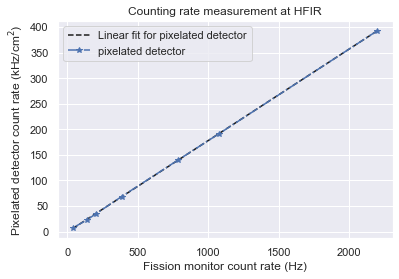
\includegraphics[width=\textwidth, height=3cm]{images/counting_rate_HFIR.png}
  \scriptsize HFIR
  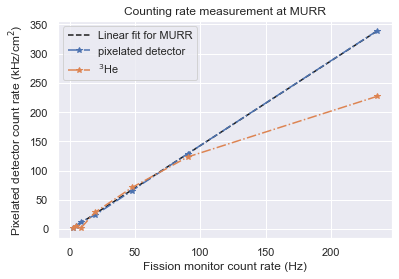
\includegraphics[width=\textwidth, height=3cm]{images/counting_rate_MURR.png}
  MURR
  \end{column}
  \begin{column}{0.33\textwidth}
  Gamma sensitivity
  \centering
  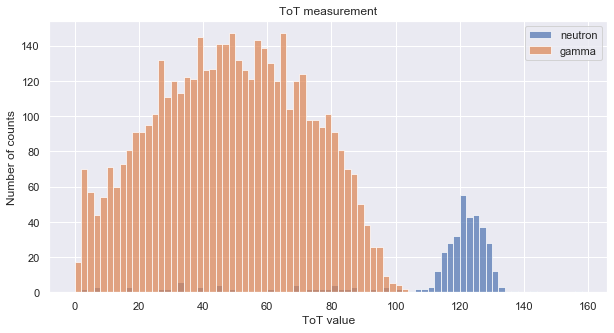
\includegraphics[width=\textwidth, height=3cm]{images/roughness3.png}
  \scriptsize 6 $\times$ 6 mm$^2$ 
  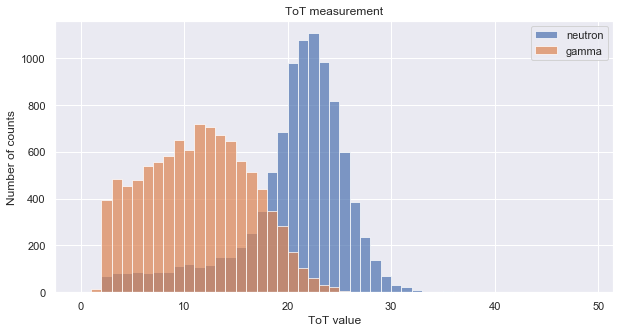
\includegraphics[width=\textwidth, height=3cm]{images/spectra3.png}
  1 $\times$ 1 mm$^2$
  MURR
  \end{column}
  \begin{column}{0.3\textwidth}
  \centering
  Active area \\
  \
  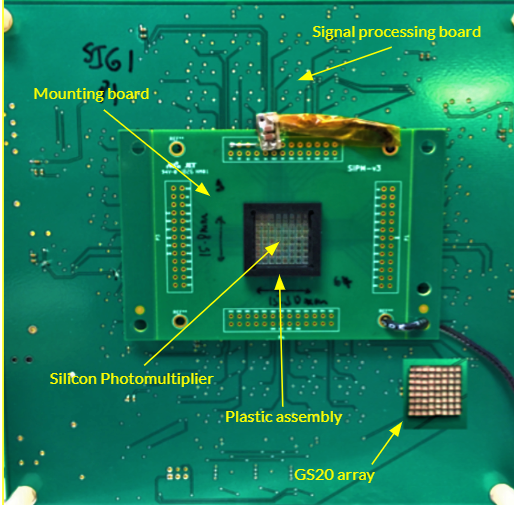
\includegraphics[width=\textwidth, height=3cm]{images/signal_processing_board.PNG}
  \raggedright \scriptsize Requires rearrangement of electronic configuration for scale-up 
  without introducing dead space within the active area of the detector \\
  \ \\
  Exploring commercially available SiPM readout systems.
  \vspace{0.4cm}
  \end{column}
  \end{columns}
  \end{center}
\end{frame}

\section{\scshape Current Work}

\begin{frame}[c]
\frametitle{Geant4 simulation}
  Scintillator studies and literature reviews
\end{frame}

\begin{frame}[c]
\frametitle{SiPM Readout System}
  
  \begin{block}{Comparison}
  \centering
  \begin{tabular}{@{}l l l}
  \hline
  Company & CAEN & Petsys \\
  \hline
  Module Name & A5202 + DT5215 & TOF ASIC evaluation kit \\
  ASIC chip & CITIROC-1A (x2) & TOFPET ASIC \\
  Channel/ASIC chip & 32 & 64 \\
  Dynamic range & 400 pC & 1500 pC \\
  Maximum channel hit rate & 20 MHz & 600 kHz  \\
  Max output data rate & 6.25 Gb/s & 3.2 Gb/s \\
  Acquisition modes & PHA, TOT & PHA, TOT, TOF \\
  % Price per unit & & \$14,000 USD\\
  % Dimension per unit & 60 mm $\times$ 15 mm & \\
  Availability & Coming soon & In stock \\
  \hline
  \end{tabular}
  \end{block}
\end{frame}

\begin{frame}
\frametitle{Board Layout}
 Printed circuit board (PCB) layout for SiPM connector. Some SiPM comes with a connector, some comes with ball grid array (BGA). \\
\ \\
  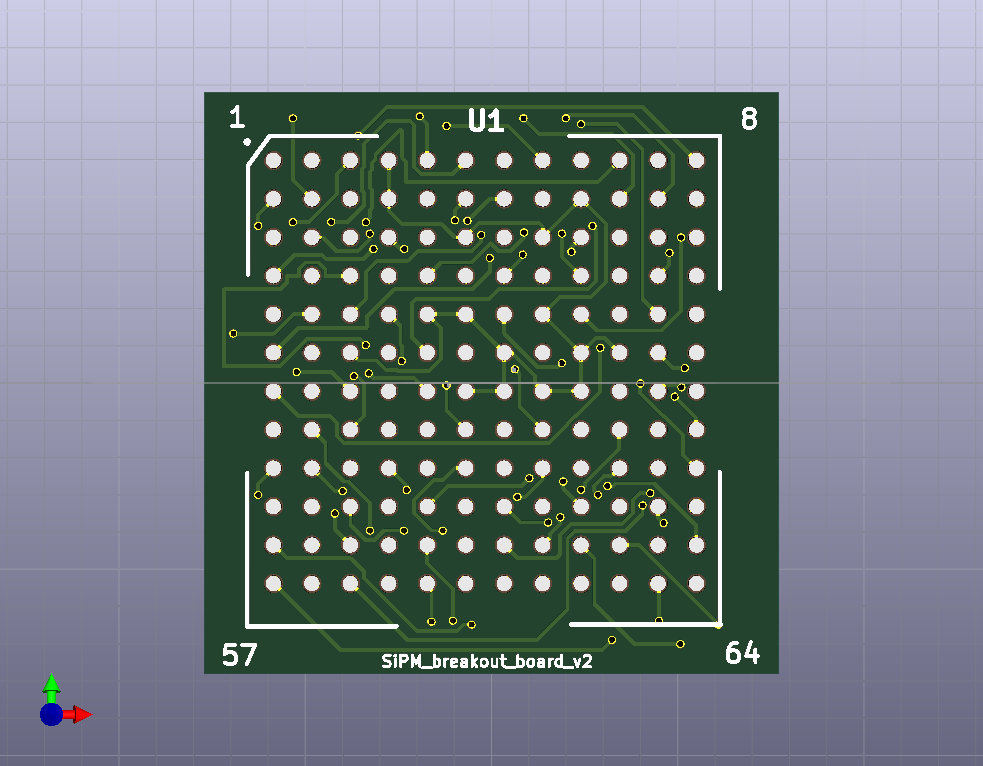
\includegraphics[width=0.49\textwidth]{images/pcb_sipm_front.png}
  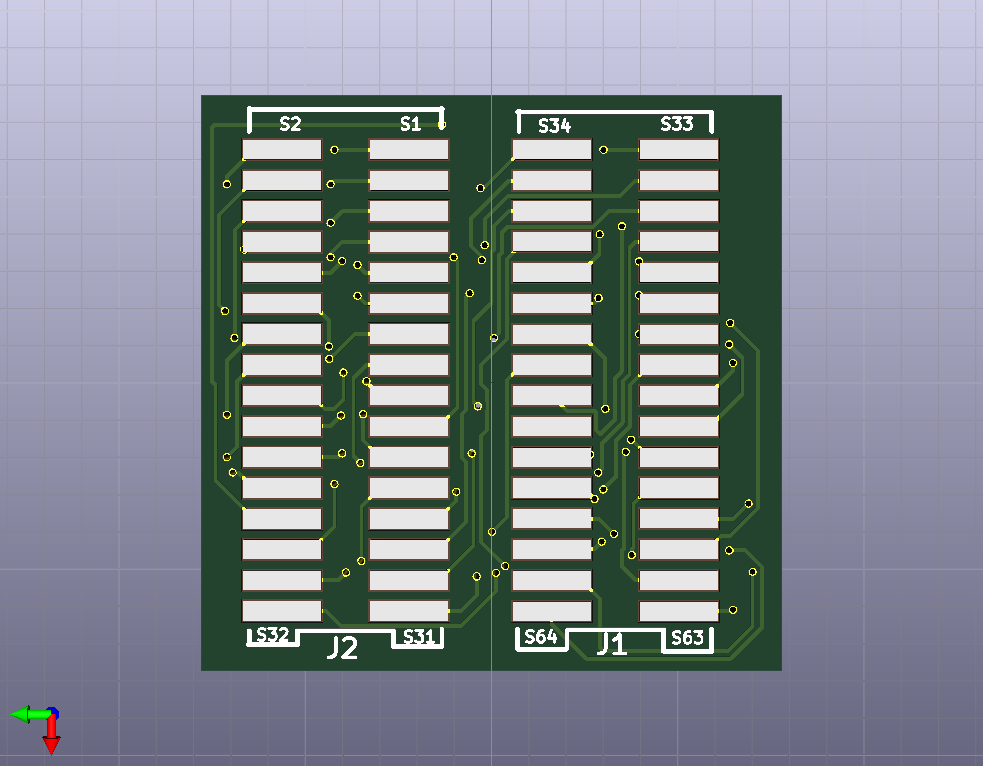
\includegraphics[width=0.49\textwidth]{images/pcb_sipm_back.png}
\end{frame}


\section{\scshape Future Work}

\begin{frame}[c]
\frametitle{This Summer}
Goals:
  \begin{itemize}
    \item Wrap up Geant4 simuation on GS20, and compare results with experimental results
    \item Once the SiPM readout system is finalized, lay out the connector board that interfaces the SiPMs with the readout system.
    \item Work on a peer-reviewed journal on the latest work and upgrades on the detector prototype.
  \end{itemize}

Possible work:
  \begin{itemize}
    \item Explore other scintillators or photosensors as alternatives
    \item Explore other signal processing techniques to improve the neutron-gamma discrimination of the detector
    \item Improve our DAQ software 
  \end{itemize}
\end{frame}

% \frame[noframenumbering, plain]{\frametitle{References}
% \tiny{\bibliographystyle{plain}}
% \bibliography{bib/bib}
% }

% \appendix

% \section{Backup Slides}

\begin{frame}[noframenumbering, plain]
  \vspace{3cm}
  \centering
  Thank you for your time!
  \vspace{3cm}
\end{frame}

\end{document}